\documentclass[
]{jss}

\usepackage[utf8]{inputenc}

\providecommand{\tightlist}{%
  \setlength{\itemsep}{0pt}\setlength{\parskip}{0pt}}

\author{
Lars van der Laan\\University of Washington, Seattle/Statistics
}
\title{\pkg{causalglm}: A \pkg{tlverse} \proglang{R} package for interpretable
and robust causal inference for heterogeneous treatment effects using
generalized linear working models and targeted machine-learning.}

\Plainauthor{Lars van der Laan}
\Plaintitle{causalglm: A tlverse R package for interpretable and robust causal
inference for heterogeneous treatment effects using generalized linear
working models and targeted machine-learning.}
\Shorttitle{\pkg{causalglm}: Interpretable and Robust Causal Inference for
Heterogeneous Treatment Effects}


\Abstract{
Generalized linear models are widely-used and interpretable methods for
learning heterogeneous treatment effects. However, generalized linear
models methods, as commonly used in practice, make strong parametric
assumptions on components of the data-generating distribution that are
not directly of interest for the causal question at hand. Notably, in
real-world settings, the relation between confounders and the outcome is
almost always unknown and may be quite complex. As a result, causal
inference based on parametric generalized linear models can be very
biased and even misleading, especially when the model is not chosen a
priori. Moreover, in high dimensional settings, generalized linear
models and their inference breaks down and alternative methods like
lasso and elastic-net regression do not easily provide inference. In
this article, we present the \proglang{R} package \pkg{causalglm} that
implements nonparametrically robust causal inference for user-specified
generalized linear working (or approximate) models for heterogeneous
treatment effects. The user-specified parametric model is viewed as an
approximation of the true nonparametric treatment-effect estimand and an
interpretable causal estimand is defined as the nonparametric projection
of this true estimand onto the working model, thereby allowing for
estimates that are causally interpretable and valid inference under a
nonparametric statistical model. These methods utilize targeted maximum
likelihood estimation and therefore can leverage adaptive
machine-learning algorithms for estimation and variable selection of
nonparametric nuisance components of the data-distribution. For binary,
categorical and continuous treatments, this package supports
nonparametric causal inference for user-specified parametric working
models of the estimands: the conditional average treatment effect, the
conditional relative risk, the conditional odds ratio, and more.
Nonparametric-robust causal inference for working marginal structural
models are also supported. In addition, a specialized lasso-based method
is implemented, allowing for robust post-confounder-selection causal
inference in very high dimensions. These methods are implemented using
the powerful \pkg{tlverse} machine-learning (\pkg{sl3}) and generalized
targeted learning (\pkg{tmle3}) ecosystem.
}

\Keywords{keywords, not capitalized, \proglang{Java}}
\Plainkeywords{keywords, not capitalized, Java}

%% publication information
%% \Volume{50}
%% \Issue{9}
%% \Month{June}
%% \Year{2012}
%% \Submitdate{}
%% \Acceptdate{2012-06-04}

\Address{
    Lars van der Laan\\
    University of Washington, Seattle/Statistics\\
    University of Washington, Seattle\\
Department of Statistics\\
  E-mail: \email{vanderlaanlars@yahoo.com}\\
  URL: \url{https://tlverse.org/causalglm/}\\~\\
  }

% Pandoc syntax highlighting

% Pandoc citation processing


\usepackage{amsmath} \usepackage{amsfonts}

\DeclareMathOperator{\logit}{logit}
\DeclareMathOperator{\argmin}{argmin}
\DeclareMathOperator{\argmax}{argmax}
\DeclareMathOperator{\expit}{expit}

\begin{document}

\hypertarget{introduction-to-causalglm}{%
\section{Introduction to causalglm}\label{introduction-to-causalglm}}

In the search for answers to causal questions, assuming parametric
models can be dangerous. With even a seemingly small amount of
confounding and model misspecificaton, they can give biased answers. One
way of mitigating this challenge is to only parametrically model the
feature of the data-generating distribution that you care about. It is
not even necessary to assume your parametric model is correct! Instead,
view it as a ``working'' or ``approximation'' model and define your
estimand as the best causal approximation of the true nonparametric
estimand with respect to your parametric working model. This allows for
causal estimates and robust inference under no parametric assumptions on
the functional form of any feature of the data generating distribution.
Alternatively, you can assume a semiparametric model that only assumes
the parametric form of the relevant part of the data distribution is
correct. Let the data speak for itself and use machine-learning to model
the nuisance features of the data that are not directly related to your
causal question. It is in fact possible to get robust and efficient
inference for causal quantities using machine-learning. Why worry about
things that don't matter for your question? It is not worth the risk of
being wrong.

\pkg{causalglm} is an all-purpose and user-friendly package for
interpretable and robust causal inference for heterogeneous treatment
effects using generalized linear working model and machine-learning.
Unlike parametric methods based on generalized linear models and
semiparametric methods based on partially-linear models, the methods
implemented in \pkg{causalglm} do not assume that any user-specified
parametric models are correctly specified. That is, \pkg{causalglm} does
not assume that the true data-generating distribution satisfies the
parametric model. Instead, the user-specified parametric model is viewed
as an approximation or ``working model'', and an interpretable estimand
is defined as a projection of the true conditional treatment effect
estimand onto the working model. Moreover, \pkg{causalglm}, unlike
\pkg{glm}, only requires a user-specified parametric working model for
the causal estimand of interest. All nuisance components of the
data-generating distribution are left unspecified and data-adaptively
learned using machine-learning. Thus, \pkg{causalglm} provides not only
nonparametrically robust inference but also provides estimates
(different from \pkg{glm}) for causally interpretable estimands that
maximally adjust for confounding. To allow for valid inference with the
use of variable-selection and machine-learning, Targeted Maximum
Likelihood Estimation (van der Laan, Rose, 2011) is employed.

By providing inference under a fully nonparametric statistical model, as
opposed to a parametric or even semiparametric statistical model,
\pkg{causalglm} gains the following features:

\begin{enumerate}
\item No model selection bias: Users can specify as many incompatible parametric working models for the treatment effect estimands as desired and obtain valid inference even when the models are incorrect. 
\item Causal estimands: The estimands estimated can be meaningfully interpreted as causal parameters (e.g. a best linear approximation) even when the working model is incorrect. Moreover, the working-model-based estimands are invariant to the level of confounding in the data. Two different studies with different levels of confounding and different treatment-assignment probabilities will estimate the same target parameter.
\item Adaptive variable-selection techniques and machine-learning can be used to adjust for confounding, thus allowing for maximal confounding bias reduction and robust inference in both low, high and very high dimensions.
\end{enumerate}

\pkg{causalglm} consists of the following functions.

\begin{enumerate}
\item `npglm` for robust nonparametric inference of user-specified working-models for conditional treatment effects with binary and categorical treatments.
\item `msmglm` for robust nonparametric inference of user-specified working marginal structural models for marginalized conditional treatment effects with binary and categorical treatments.
\item `contglm` for robust nonparametric inference of user-specified working models for conditional treatment effects with continuous treatments.
\item `spglm` for semiparametric inference of assumed-to-be correctly-specified parametric models for conditional treatment effects with binary treatments.
\item `causalglmnet` for semiparametric inference of assumed-to-be correctly-specified parametric models for conditional treatment effects in high dimensions with binary treatments.
\end{enumerate}

\section{Data-Structure and treatment-effect estimands}

We will mainly consider the point-treatment data-structure
\(O = (W,A,Y)\) where \(W\) represents a vector of baseline covariates
(i.e.~possible confounders), \(A\) is a binary, categorical or
continuous treatment assignment, and \(Y\) is some outcome variable. As
an example, for a given observation \(O\), \(W\) could be measurements:
age, sex, a risk-score, location, income; \(A\) could be categorical and
take the value \(a\) if the individual receives treatment \(a\) and
\(0\) if they do not receive any treatment; and \(Y\) is a binary or
continuous variable that captures the effect of the treatment.
Additionally, for the marginal structural model estimands, we will also
consider a subvector of baseline variables \(V \subset W\). For the goal
of assessing heterogeneity of the treatment effect, there are a number
of popular estimands that are implemented in this package:

\noindent The conditional average treatment effect (CATE):
\begin{equation}
CATE_{a}(w) := E[Y|A=a,W=w] - E[Y|A=0, W=w],
\end{equation} which is an additive measure of the effect of the
treatment (\(A=a\)) relative to no treatment \((A=0)\).

\vspace{0.5cm}

\noindent The conditional odds ratio (OR) for when \(Y\) is binary:
\begin{equation}
OR_a(w) := \frac{P(Y=1|A=a,W=w)/P(Y=0|A=1,W=w)}{P(Y=1|A=0,W=w)/P(Y=0|A=0,W=w)}
\end{equation}

\vspace{0.5cm}

\noindent The conditional relative risk (RR) for when \(Y\) is
nonnegative (e.g.~a binary or count variable): \begin{equation}
RR_a(w) := \frac{E[Y|A=a,W=w]}{E[Y|A=0,W=w]},
\end{equation} which is a relative measure of the effect of the
treatment (\(A=a\)) relative to no treatment \((A=0)\).

\vspace{0.5cm}

\noindent In some application, non-contrast measures like the
conditional treatment-specific mean (TSM) may be of interest:
\begin{equation}
TSM_a(w) := E[Y|A=a,W=w].
\end{equation}

Often, we are only interested in the treatment effect as a function of a
subset \(V\) of the collected variables \(W\). In such settings, we
would still like to adjust for all variables \(W\) to minimize
confounding bias but only wish to model the treatment effect as a
function of \(V\). Marginal structural models provide a rich class of
causal estimands that accomplish this. Key estimands considered in this
package are

\noindent The \(V\)-specific conditional average treatment effect
(\(V\)-CATE): \begin{equation}
E[CATE_{a}(W)|V=v] := E\left\{ E[Y|A=a,W] - E[Y|A=0, W] \mid V =v\right\}.
\end{equation}

\vspace{0.5cm}

\noindent The \(V\)-specific conditional average treatment effect among
the treated (\(V\)-CATT): \begin{equation}
E[CATE_{a}(W)|V=v, A=a] := E\left\{ E[Y|A=a,W] - E[Y|A=0, W] \mid V =v, A =a\right\}.
\end{equation} \vspace{0.5cm}

\noindent The \(V\)-specific conditional relative risk (\(V\)-RR) for
when \(Y\) is nonnegative (e.g.~a binary or count variable):
\begin{equation}
E[RR_a(W)|V=v] := \frac{E[E[Y|A=a,W] \mid V=v]}{E[E[Y|A=0,W] \mid V=v]}.
\end{equation}

\vspace{0.5cm}

\noindent The \(V\)-specific conditional treatment-specific mean
(\(V\)-TSM) may be of interest: \begin{equation}
E[TSM_a(W) \mid V =v ] := E[E[Y|A=a,W] \mid V = v].
\end{equation}

\subsection{Conventional estimators using parametric generalized linear models and semiparametric generalized partially-linear models}

In order to estimate the estimands of the previous section, parametric
generalized linear models are often employed (e.g.~the R package
\pkg{glm}). For the CATE, the following linear regression model is often
used:
\[E[Y|A, W=w] =    \beta_1^T \underline{f}_1(w) \cdot A + \beta_2^T \underline{f}_2(w),\]
where \(\underline{f}_1(w),\, \underline{f}_2(w)\) are user-specified
vector-valued functions that encode the parametric model. This model is
equivalent to assuming both the nuisance linear model
\[E[Y|A=0,W=w] =  \beta_2^T \underline{f}_2(w) \] and target linear
model \[CATE(w) = \beta_1^T \underline{f}_1(w).\] An immediate drawback
of this model is that strong parametric assumptions are made not only on
the target estimand \(CATE(w)\) but also on the orthogonal nuisance
function \(E[Y|A=0,W]\) which is not meaningfully related to the
estimand of interest\$. As a consequence, unnecessary assumptions are
made that do not provide any meaningful benefit in interpretability and
can only bias the estimates for the target estimand.

A more robust way of estimating the CATE is to assume a semiparametric
model. Specifically, we could assume the partially-linear linear-link
regression model which only assumes that
\[CATE(w) = \beta^T \underline{f}(w).\] Thus, only the relevent feature
of the data-generating distribution, the actual estimand, is modeled
parametrically. This assumption is equivalent to the regression model:
\[E[Y|A,W=w] = A \cdot \beta^T \underline{f}(w) + h_0(w),\] where
\(h_0(w) := E[Y|A=0,W]\) is left unspecified. While the semiparametric
model makes assumptions much weaker than the parametric model, it still
makes strong parametric assumptions on the target estimand. In
particular, the semiparametric still requires apriori correctly
specifying a parametric model for the estimand for valid inference and
therefore suffers from issues like model selection bias. Also, it is not
easy to generalize the estimators based on these models to marginal
structural model estimands.

Before going to the other estimands, it will be useful to generalize the
parametric and semiparametric model considered above for general link
functions. For a given monotone link function
\(g: \mathbb{R} \rightarrow \mathbb{R}\), the generalized linear model
assumes
\[g(E[Y|A,W=w]) = \beta_1^T \underline{f}_1(w) \cdot A + \beta_2^T \underline{f}_2(w),\]
where \(\underline{f}_1(w),\, \underline{f}_2(w)\) are user-specified
vector-valued functions that encode the parametric model. The
generalized partially linear model assumes
\[g(E[Y|A,W=w]) = A \cdot \beta^T \underline{f}(w)  + g(E[Y|A=0,W]),\]
where \(\underline{f}(w)\) is a user-specified vector-valued function
that encodes a parametric model for the estimand of interest and
\(E[Y|A=0,W]\) is left unspecified.

The CATE-based models we just considered correspond with the identity
link function \(g(x) := x\). The conditional odds ratio can be estimated
using the parametric logistic regression model and semiparametric
partially-linear logistic regression model, which correspond with the
logistic link \(g(p) = \frac{p}{1-p}\). The parametric logistic
regression model is equivalent to assuming both the nuisance logistic
model
\[\logit \left\{ E[Y|A=0,W=w] \right\} =  \beta_2^T \underline{f}_2(w) \]
and target log-linear model
\[\log OR(w) = \beta_1^T \underline{f}_1(w).\] The semiparametric method
only assumes that \(\log OR(w) = \beta^T \underline{f}(w).\)

\noindent For estimation of the conditional relative risk, the link
function is chosen to be \(g(x) = \log x\), which corresponds with the
parametric and partially-linear log-linear models. The parametric
log-linear model is equivalent to assuming both the nuisance log-limear
model
\[\log \left\{ E[Y|A=0,W=w] \right\} =  \beta_2^T \underline{f}_2(w) \]
and target log-linear model
\[\log RR(w) = \beta_1^T \underline{f}_1(w).\] The semiparametric
partially-linear log-linear model only assumes that
\[\log RR(w) = \beta^T \underline{f}(w)\] and leaves \(E[Y|A=0,W]\)
unspecified. Both the conditional odds ratio and relative risk
parametric and semiparametric models suffer from similar issues as the
CATE models.

\section{Nonparametric working-model-based estimands for model-free inference}

In this section, we introduce nonparametrically-defined estimands based
on projections of the true conditional treatment-effect estimands onto
parametric working-models. We consider the estimands based on binary and
categorical treatments separately from the estimands based on continuous
treatments.

\subsection{Working-model-based nonparametric estimands for binary or categorical treatments}\label{section::estimandNPcat}

Let \(a\) be a given treatment level of \(A\) that is of interest.
Consider the least-squares projection estimand, \begin{equation}
\beta_{a,CATE} := \argmin_{\beta} E\left(CATE_a(W) - \beta^T \underline{f}(W) \right)^2 \label{eqn::estimandNPCATE}
\end{equation} where \(\beta_{a,CATE}^T \underline{f}(w)\) is the best
linear approximation of the true \(CATE_a(W)\) relative to the average
squared-error loss. Clearly, when the parametric working-model
\(\beta^T \underline{f}(w)\) is correctly specified, \(\beta_{a,CATE}\)
reduces to the same estimand considered by the parametric and
semiparametric methods. When the working-model is incorrect, the causal
interpretation of \(\beta_{a,CATE}\) as an approximation is clear.
Importantly, \(\beta_{a,CATE}\) is invariant with respect to the
treatment-assignment probability \(P(A=a|W)\), which crucially ensures
this nonparametric estimand is not affected by confounding.

This same estimand also has the property that it reduces to the best
approximation of a \(V-specific\) marginal structural working model when
the parametric form is lower-dimensional and satisfies
\(\underline{f}(W=w) \equiv \underline{f}(V=v)\). To see this, note that
minimizing \(E\left(CATE_a(W) - \beta^T \underline{f}(V) \right)^2\) is
equivalent to minimizing
\(E\left\{\left( \beta^T \underline{f}(V) \right)^2 - 2 \beta^T \underline{f}(V)CATE_a(W) \right\}\).
Applying the law of iterated conditional expectations and applying the
equivalence in reverse, we find
\[\argmin_{\beta} E\left(CATE_a(W) - \beta^T \underline{f}(V) \right)^2 = \argmin_{\beta} E\left(E[CATE_a(W)|V] - \beta^T \underline{f}(V) \right)^2.\]
Thus, the estimand \(\beta_{a,CATE}\) has the powerful property of
automatically reducing to the least-squares projection of the true
\(V\)-specific marginal structural CATE model onto the user-specified
working model \(\beta^T \underline{f}(V=v)\). This allows for the
development of a single estimator/method that simultaneously allows for
estimates and inference for both conditional estimands and marginal
structual model estimands.

A notable special case if when \(\underline{f}(w) := 1\) is taken as the
intercept model. We then find
\[\beta_{a,CATE} = \argmin_{\beta} E\left(CATE_a(W) - \beta \right)^2 = E[CATE(W)] = E[E[Y|A=a,W]] - E[E[Y|A=0,W]]\]
which is exactly the nonparametric marginal average treatment effect
estimand!

Based on the least-squares projection, we can define natural
working-model estimands for the conditional treatment-specific mean
(TSM) and the conditional average treatment effect among the treated:

\begin{equation}
\beta_{a,CATT} := \argmin_{\beta} E\left\{\left(CATE_a(W) - \beta^T \underline{f}(W) \right)^2 \mid A =a \right\}, \label{eqn::estimandNPCATT}
\end{equation} \begin{equation}
\beta_{a,TSM} := \argmin_{\beta} E\left(E[Y|A=a,W]- \beta^T \underline{f}(W) \right)^2.
\label{eqn::estimandNPTSM}
\end{equation}

Both these working model estimands similarly reduce to projections of
the true marginal structural model estimands for lower dimensional
working-models. Specifically, we have the identities
\[  \argmin_{\beta} E\left\{\left(E[CATE_a(W) - \beta^T \underline{f}(V)  \right)^2\mid A =a\right\} \]
\[=  \argmin_{\beta} E\left\{\left(E[CATE_a(W)|V, A=a] - \beta^T \underline{f}(V)  \right)^2\mid A =a\right\},\]
and
\[ \argmin_{\beta} E\left(E[Y|A=a,W]- \beta^T \underline{f}(V) \right)^2 =  \argmin_{\beta} E\left(E[E[Y|A=a,W]|V]- \beta^T \underline{f}(V) \right)^2.\]

Next, we consider the nonparametric working-model-based estimands for
conditional relative risk (RR) which will utilize projections based on
the poisson (log-linear) log-likelihood loss function. Specifically,
define the poisson-likelihood-type projection estimand: \begin{equation}
\beta_{a,RR} := \argmin_{\beta} E \left\{E[Y|A=0,W] \cdot e^{\beta^T \underline{f}(W)} - E[Y|A=a,W] \cdot \beta^T \underline{f}(W) \right\}.
\label{eqn::estimandNPRR}
\end{equation} It can be verified when \(\beta^T \underline{f}(W)\) is
correctly specified for the conditional relative risk that
\(\beta_{a,RR}\) indeed reduces to the true coefficient vector. While
this estimand is motivated by the poisson and log-linear loss functions,
we note that it is well-defined nonparametrically and we make no
assumptions on the error distribution of our outcome. One reason for
choosing this projection to define the estimand is because it reduces to
the projection of a marginal structural model for the relative treatment
effect when \(\underline{f}(W=w) \equiv \underline{f}(V=v)\) is
lower-dimensional. Specifically, we have the identity
\[\argmin_{\beta} E \left\{E[Y|A=0,W] \cdot e^{\beta^T \underline{f}(V)} - E[Y|A=a,W] \cdot \beta^T \underline{f}(V) \right\}\]
\[= \argmin_{\beta} E \left\{E[E[Y|A=0,W]|V] \cdot e^{\beta^T \underline{f}(V)} - E[E[Y|A=a,W]V] \cdot \beta^T \underline{f}(V) \right\},\]
where the right-hand side is the log-linear projection of the
\(V\)-specific marginalized conditional relative risk function
\(\frac{E[E[Y|A=a,W]V]}{E[E[Y|A=0,W]V]}\) onto the working-model
\(\beta^T \underline{f}(V=v)\). Under the special case where the
intercept working model \(\underline{f}(w) := 1\) is used, we have
\[\beta_{a,RR} = \frac{E[E[Y|A=a,W]]}{E[E[Y|A=0,W]]}\], which is the
nonparametric marginal relative risk.

Finally, we present a working-model for the conditional odds ratio based
on the logistic-link log-likelihood projection. First, define the
working-model
\[P_{\beta}(Y=1|A=a,W) :=  \expit\left\{\beta^T \underline{f}(W)  + \logit(P(Y=1,A=0,W))\right\}.\]
Consider the estimand, \begin{equation}
\beta_{a,OR} = \argmin_{\beta} -1 \cdot E\bigg\{P(Y=1|A=a,W)\log \left\{P_{\beta}(Y=1|A=a,W)\right\} $$
$$+ P(Y=0|A=a,W)\log \left\{1-P_{\beta}(Y=1|A=a,W)\right\} \bigg\},
\label{eqn::estimandNPOR}
\end{equation} which is the log-likelihood projection of
\(P(Y=1|A=a,W)\) onto the working model \(P_{\beta}(Y=1|A=a,W)\). Since
\(P_{\beta}(Y=1|A=0,W) = P_{\beta}(Y=1|A=0,W)\) is correctly specified,
this projection is targeted towards \(\beta^T \underline{f}(w)\) which
is a log-linear working model for the conditional odds ratio
\(OR_a(w)\). This estimand only reduces to a \(V\)-specific marginal
structural working model conditional odds ratio estimand when
\(P(Y=1|A=0,W) = P(Y=1|A=0,V)\), which may not be true in practice but
is still a useful property to have.

\subsection{Robust working-model-based nonparametric estimands for continuous treatments}\label{section::estimandNPcont}

When \(A\) represents a continuous or ordered numeric treatment, we
utilize working-models that also model the treatment-dependence of the
conditional treatment effect estimand. For computational reasons, it is
beneficial to solely consider least-squares-type projections for all
estimands. Specifically, for a given link function
\(g:\mathbb{R} \rightarrow \mathbb{R}\), we consider working models of
the form
\[g(E[Y|A=a,W=w]) - g(E[Y|A=0,W=w]) = 1(a>0)\cdot \beta_0^T \underline{f}_0(w) +  a \cdot \beta_1^T \underline{f}_1(w),\]
where we assume that the treatment \(A\) is nonnegative and \(A=0\)
encodes the control arm. The first term models discontinuous treatment
effects associated with being either treated or not. The second term
models continuous or dosage-dependent treatment effects. We define a
rich class of nonparametrically-defined working-model-based estimands
via the least-squares projection
\[(\beta_{0,g}, \beta_{1,g}) := \argmin_{\beta_0, \beta_1} E \left\{ g(E[Y|A,W]) - g(E[Y|A=0,W])  - 1(A>0)\cdot \beta_0^T \underline{f}_0(W) +  A \cdot \beta_1^T \underline{f}_1(W)\right\}^2.\]

For the identity link \(g(x) := x\), we obtain as estimand the
least-squares projection of the true CATE
\[ (\beta_{0,CATE}, \beta_{1,CATE}) := \argmin_{\beta_0, \beta_1} E \left\{ CATE_A(W)  - 1(A>0)\cdot \beta_0^T \underline{f}_0(W) +  A \cdot \beta_1^T \underline{f}_1(W)\right\}^2.\]

For the log link \(g(x) = \log x\), we obtain as estimand the
least-squares projection of the true conditional log RR
\[ (\beta_{0,RR}, \beta_{1,RR}) :=  \argmin_{\beta_0, \beta_1} E \left\{ \log RR_{A}(W)  - 1(A>0)\cdot \beta_0^T \underline{f}_0(W) +  A \cdot \beta_1^T \underline{f}_1(W)\right\}^2.\]

For the log-odds link \(g(p) = \log p - \log (1-p)\), we obtain as
estimand the least-squares projection of the true conditional log OR
\[ (\beta_{0,OR}, \beta_{1,OR}) :=  \argmin_{\beta_0, \beta_1} E \left\{ \log OR_{A}(W)  - 1(A>0)\cdot \beta_0^T \underline{f}_0(W) +  A \cdot \beta_1^T \underline{f}_1(W)\right\}^2.\]

\section{Model-robust causal inference with npglm and msmglm}

\textit{npglm} is one of the main functions of \pkg{causalglm} and
implements statistically efficient estimators for the
nonparametrically-defined working-model-based conditional treatment
effect estimands defined in Section \ref{section::estimandNPcat}.
\textit{msmglm} is a specialized wrapper function for \textit{npglm}
that focuses on marginal structural working model estimation and
provides additional plotting features for such models. Both methods have
user-friendly front-end and only require the following arguments:

\begin{enumerate}
\item \textit{formula} : An R formula object that specifies a parametric working model for the conditional treatment-effect estimand.
\item \textit{data}: A data.frame containing the baseline, treatment and outcome variables.
\item $W$: A character vector containing the names of the variables in \textit{data} for which to adjust (i.e. possible confounders).
\item $A$:  A character string giving the name of the treatment variable of interest in \textit{data}.
\item $Y$: A character string giving the name of the outcome variable of interest in \textit{data}.
\item \textit{estimand}: A character string specifying the estimand - \textit{CATE, OR, RR, CATT, TSM}.
\end{enumerate}

Additionally, the following optional arguments are useful.

\begin{enumerate}
\item \textit{learning\_method} : A character string specifying one of the built-in machine-learning algorithms for nuisance function estimation. The nuisance functions are $P(A=1|W)$ and $E[Y|A,W]$. By default, the Highly Adaptive Lasso (Benkeser, van der Laan, 2016) using the package \pkg{tlverse/hal9001} (Coyle et al., 2021) is used.
\item \textit{treatment\_level}: A value/level of the treatment $A$ that encodes the treatment arm of interest. (useful for categorical treatments )
\item \textit{control\_level}: A value/level of the treatment $A$ that encodes the control arm. (useful for categorical treatments)
\item $sl3\_Learner\_A$: A \pkg{sl3} learner object that specifies a custom estimator for the treatment-assignment probability $P(A=1|W)$. (Overrides \textit{learning\_method})
\item $sl3\_Learner\_Y$: A \pkg{sl3} learner object that specifies a custom estimator for the true outcome conditional mean $E[Y|A,W]$. (Overrides \textit{learning\_method})
\end{enumerate}

Let's see npglm and msmglm in action! Let us start with estimation of
the CATE estimand as defined by equation \label{eqn::estimandNPCATE}. We
will use the following simulated dataset. Note the true conditional
average treatment effect is
\(CATE_1(W) = 1 + W_1 + 2 \cdot W_1^2 + W_2\).

\begin{CodeChunk}
\begin{CodeOutput}
Loading required package: sl3
\end{CodeOutput}
\begin{CodeOutput}
Loading required package: hal9001
\end{CodeOutput}
\begin{CodeOutput}
Loading required package: Rcpp
\end{CodeOutput}
\begin{CodeOutput}
hal9001 v0.4.0: The Scalable Highly Adaptive Lasso
note: fit_hal defaults have changed. See ?fit_hal for details
\end{CodeOutput}
\begin{CodeOutput}
Loading required package: data.table
\end{CodeOutput}
\begin{CodeOutput}
Loading required package: R6
\end{CodeOutput}
\begin{CodeOutput}
Loading required package: tmle3
\end{CodeOutput}
\begin{CodeOutput}

Attaching package: 'tmle3'
\end{CodeOutput}
\begin{CodeOutput}
The following object is masked from 'package:sl3':

    loss_loglik_binomial
\end{CodeOutput}
\end{CodeChunk}

Let us specify a correct working model for the CATE.

\begin{CodeChunk}
\begin{CodeInput}
R> formula_CATE <- ~ poly(W1, degree = 2, raw = TRUE) + W2
R> output <- npglm(
+       formula_CATE, 
+       data,
+       W = c("W1", "W2"), A = "A", Y = "Y",
+       estimand = "CATE", 
+       learning_method = "HAL", # Default
+       verbose = FALSE
+       )
\end{CodeInput}
\end{CodeChunk}

``output'' is a \textit{npglm} fit object which supports a number of
useful extraction methods. Using the ``summary'' function, we can
extract coefficient estimates, p-values, and 95\% confidence intervals.
Using the ``predict'' function, we can obtain individual-level treatment
effect predictions with 95\% confidence intervals.

\begin{CodeChunk}
\begin{CodeInput}
R> summary(output)
\end{CodeInput}
\begin{CodeOutput}
A causalglm fit object obtained from npglm for the estimand CATE with formula: 
CATE(W) = 1.02 * (Intercept) + 0.979 * poly(W1, degree = 2, raw = TRUE)1 + 1.98 * poly(W1, degree = 2, raw = TRUE)2 + 1.05 * W2

Coefficient estimates and inference:
   type                             param  tmle_est         se     lower
1: CATE                       (Intercept) 1.0209493 0.05471526 0.9137094
2: CATE poly(W1, degree = 2, raw = TRUE)1 0.9786549 0.06346015 0.8542753
3: CATE poly(W1, degree = 2, raw = TRUE)2 1.9774734 0.12547989 1.7315374
4: CATE                                W2 1.0495338 0.06382252 0.9244440
      upper  Z_score p_value
1: 1.128189 295.0297       0
2: 1.103035 243.8364       0
3: 2.223409 249.1762       0
4: 1.174624 260.0115       0
\end{CodeOutput}
\begin{CodeInput}
R> head(predict(output, data = data))[1:3,c(5,7,8,9,10)]
\end{CodeInput}
\begin{CodeOutput}
       CATE(W)    CI_left  CI_right    Z-score p-value
1  1.057501602  0.9489171 1.1660861 19.0883963 0.00000
2  0.009840597 -0.1436945 0.1633756  0.1256232 0.90003
3 -0.031330635 -0.1901844 0.1275231  0.3865697 0.69907
\end{CodeOutput}
\end{CodeChunk}

In some settings, we may only be interested in the relation between the
variable \(V := W_1\) and the treatment effect. However, we would still
like to adjust for the possible confounder \(W_2\). For this, the
\textit{msmglm} function comes in handy. Let us specify an approximate
working marginal structural model for the \(W_1\)-specific CATE.
\textit{msmglm} requires the additional specification of the argument
\(V\). The output object supports the summary and predict functions and
also supports a useful plotting function ``plot\_msm'' when \(V\) is
one-dimensional. plot\_msm plots the fit marginal structural working
model as a function of \(V\) and provides 95\% pointwise confidence
intervals.

\begin{CodeChunk}
\begin{CodeInput}
R> formula_msm <- ~ poly(W1, degree = 2, raw = TRUE)  
R> output <- msmglm(
+       formula_msm, 
+       data,
+       V = c("W1"),
+       W = c("W1", "W2"), A = "A", Y = "Y",
+       estimand = "CATE", 
+       learning_method = "mars", # Lets use multivariate adaptive regression splines instead
+       verbose = FALSE
+       )
R> summary(output)
\end{CodeInput}
\begin{CodeOutput}
A causalglm fit object obtained from msmglm for the estimand CATE with formula: 
E[CATE(W)|V] = 0.908 * (Intercept) + 0.695 * poly(W1, degree = 2, raw = TRUE)1 + 2.32 * poly(W1, degree = 2, raw = TRUE)2

Coefficient estimates and inference:
   type                             param  tmle_est        se     lower
1: CATE                       (Intercept) 0.9083540 0.1564530 0.6017118
2: CATE poly(W1, degree = 2, raw = TRUE)1 0.6948623 0.1982297 0.3063392
3: CATE poly(W1, degree = 2, raw = TRUE)2 2.3206648 0.3610101 1.6130980
      upper   Z_score p_value
1: 1.214996  91.79972       0
2: 1.083385  55.42427       0
3: 3.028232 101.63962       0
\end{CodeOutput}
\begin{CodeInput}
R> head(predict(output, data = data))[1:3,c(-1,-2,-3,-5)]
\end{CodeInput}
\begin{CodeOutput}
    CATE(W)   CI_left CI_right  Z-score    p-value
1 0.8572590 0.5540882 1.160430 5.542181 2.9873e-08
2 0.8822580 0.5758463 1.188670 5.643473 1.6665e-08
3 0.8941382 0.5874837 1.200793 5.714936 1.0975e-08
\end{CodeOutput}
\begin{CodeInput}
R> plot_msm(output)
\end{CodeInput}
\begin{CodeOutput}
Loading required package: ggplot2
\end{CodeOutput}
\begin{CodeOutput}
`geom_smooth()` using method = 'loess' and formula 'y ~ x'
\end{CodeOutput}


\begin{center}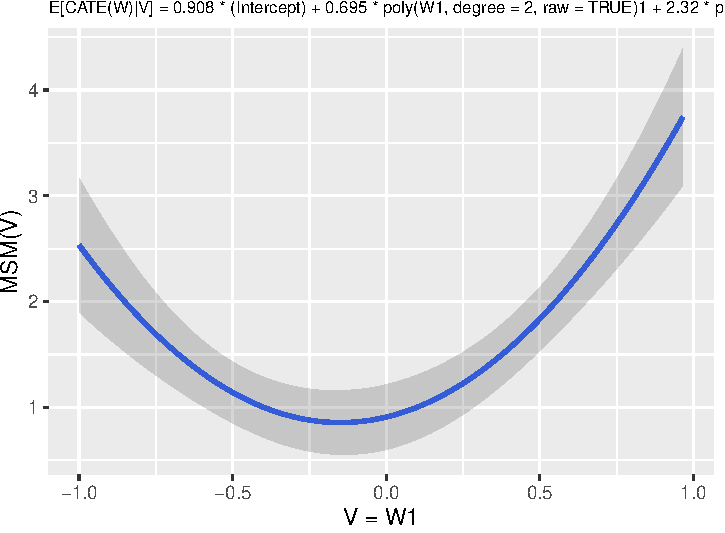
\includegraphics{causalglm_files/figure-latex/unnamed-chunk-4-1} \end{center}

\end{CodeChunk}

Now, consider a similar dataset with a categorical treatment.

\begin{CodeChunk}
\begin{CodeOutput}
Warning in A[A == 0] <- rbinom(n, size = 1, prob = plogis(W1 + W2)): number of
items to replace is not a multiple of replacement length
\end{CodeOutput}
\begin{CodeOutput}
A
 0  1  2 
65 91 94 
\end{CodeOutput}
\end{CodeChunk}

Let us compute the CATT and TSM estimands as defined in equations
\ref{eqn::estimandNPCATT} and \ref{eqn::estimandNPTSM}. Since \(A\) is
categorical, we need to specify the treatment and control levels of
interest to fully specify the estimand. Note that a single call to npglm
will fully fit all nuisance functions using machine-learning and it is
therefore a waste to recall ``npglm'' or ``msmglm'' with new treatment
and control levels. To leverage previous fits, we can pass a previous
``npglm'' or ``msmglm'' object as the ``data''. argument. The data and
variable names are extracted from the old object. This also allows us to
fit multiple different working models quickly. Let us change the
learning algorithm to CV-tuned ``xgboost''.

\begin{CodeChunk}
\begin{CodeInput}
R> # Working model for E[Y|A=1,W] - E[Y|A=0,W]
R> formula_CATT <- ~ poly(W1, degree = 3, raw = TRUE) + W2
R> output_initial <- npglm(
+       formula_CATT, 
+       data,
+       W = c("W1", "W2"), A = "A", Y = "Y",
+       estimand = "CATT", 
+       learning_method = "xgboost", # Lets use xgboost
+       treatment_level = 1, # Specify the treatment level
+       control_level = 0, # Specify the control level
+       verbose = FALSE
+       )
R> summary(output_initial)
\end{CodeInput}
\begin{CodeOutput}
A causalglm fit object obtained from npglm for the estimand CATT with formula: 
CATT(W) = 1.02 * (Intercept) + 0.294 * poly(W1, degree = 3, raw = TRUE)1 + 1.99 * poly(W1, degree = 3, raw = TRUE)2 + 1.04 * poly(W1, degree = 3, raw = TRUE)3 + 1.03 * W2

Coefficient estimates and inference:
   type                             param  tmle_est        se      lower
1: CATT                       (Intercept) 1.0221228 0.1102688  0.8059999
2: CATT poly(W1, degree = 3, raw = TRUE)1 0.2938301 0.3911505 -0.4728109
3: CATT poly(W1, degree = 3, raw = TRUE)2 1.9915965 0.2874667  1.4281720
4: CATT poly(W1, degree = 3, raw = TRUE)3 1.0357019 0.6404250 -0.2195079
5: CATT                                W2 1.0324894 0.1465707  0.7452160
      upper   Z_score p_value
1: 1.238246 146.56167       0
2: 1.060471  11.87743       0
3: 2.555021 109.54278       0
4: 2.290912  25.57034       0
5: 1.319763 111.38028       0
\end{CodeOutput}
\begin{CodeInput}
R> # Working model for E[Y|A=2,W] - E[Y|A=0,W]
R> formula_CATT <- ~ poly(W1, degree = 2, raw = TRUE) + W2
R> output <- npglm(
+       formula_CATT, 
+       data = output_initial, # replace data with previous output
+       estimand = "CATT", 
+       treatment_level = 2,  # Specify new treatment levels
+       control_level = 0,
+       verbose = FALSE
+       )
R> summary(output)
\end{CodeInput}
\begin{CodeOutput}
A causalglm fit object obtained from npglm for the estimand CATT with formula: 
CATT(W) = 1.94 * (Intercept) + 1.8 * poly(W1, degree = 2, raw = TRUE)1 + 4.22 * poly(W1, degree = 2, raw = TRUE)2 + 2.16 * W2

Coefficient estimates and inference:
   type                             param tmle_est        se    lower    upper
1: CATT                       (Intercept) 1.937332 0.1445649 1.653990 2.220674
2: CATT poly(W1, degree = 2, raw = TRUE)1 1.799968 0.1783153 1.450477 2.149460
3: CATT poly(W1, degree = 2, raw = TRUE)2 4.223237 0.3304522 3.575563 4.870911
4: CATT                                W2 2.164614 0.1683955 1.834565 2.494664
    Z_score p_value
1: 211.8904       0
2: 159.6049       0
3: 202.0723       0
4: 203.2451       0
\end{CodeOutput}
\begin{CodeInput}
R> # Lets use a different formula and reuse previous fits
R> # We can even reuse fits across npglm and msmglm
R> formula_CATT <- ~1 + W2  
R> output <- msmglm(
+       formula_CATT, 
+       data = output_initial, # replace data with previous output
+       estimand = "CATT", 
+       V = "W2",
+       treatment_level = 2,  # Specify new treatment levels
+       control_level = 0,
+       verbose = FALSE
+       )
R> summary(output)
\end{CodeInput}
\begin{CodeOutput}
A causalglm fit object obtained from msmglm for the estimand CATT with formula: 
E[CATE(W)|V, A=1] = 3.81 * (Intercept) + 1.86 * W2

Coefficient estimates and inference:
   type       param tmle_est        se   lower    upper   Z_score p_value
1: CATT (Intercept) 3.809115 0.2208943 3.37617 4.242060 272.65249       0
2: CATT          W2 1.862513 0.3674519 1.14232 2.582705  80.14359       0
\end{CodeOutput}
\end{CodeChunk}

The TSM estimand is slightly different than other methods. It does not
require specification of a control level. Instead, you can specify
multiple treatment levels and conditional treatment-specific mean
working-model estimates are returned for each level in the form of a
list of ``msmglm'' objects.

\begin{CodeChunk}
\begin{CodeInput}
R> # Marginal structural model for TSM
R> formula_TSM <- ~ 1  
R> # Code is similar for npglm
R> output <- msmglm( 
+       formula_TSM, 
+       output_initial,
+       V = c(),
+       estimand = "TSM", 
+       learning_method = "HAL", # Default
+       verbose = FALSE,
+       treatment_level = c(0,1,2) # Computes TSM for all treatment levels
+       )
R> # The output is a list of msmglm objects for each treatment level in this case.
R> output_A0 <- output[[1]]
R> output_A1 <- output[[2]]
R> output_A2 <- output[[3]]
R> summary(output_A0)
\end{CodeInput}
\begin{CodeOutput}
A causalglm fit object obtained from msmglm for the estimand TSM with formula: 
E[TSM(W)|V] = 0.0651 * E[Y_{A=0}]: (Intercept)

Coefficient estimates and inference:
   type                   param   tmle_est         se      lower     upper
1:  TSM E[Y_{A=0}]: (Intercept) 0.06513606 0.09367549 -0.1184645 0.2487366
    Z_score p_value
1: 10.99425       0
\end{CodeOutput}
\begin{CodeInput}
R> summary(output_A1)
\end{CodeInput}
\begin{CodeOutput}
A causalglm fit object obtained from msmglm for the estimand TSM with formula: 
E[TSM(W)|V] = 1.8 * E[Y_{A=1}]: (Intercept)

Coefficient estimates and inference:
   type                   param tmle_est        se    lower    upper  Z_score
1:  TSM E[Y_{A=1}]: (Intercept) 1.800613 0.1174023 1.570509 2.030717 242.5012
   p_value
1:       0
\end{CodeOutput}
\begin{CodeInput}
R> summary(output_A2)
\end{CodeInput}
\begin{CodeOutput}
A causalglm fit object obtained from msmglm for the estimand TSM with formula: 
E[TSM(W)|V] = 3.46 * E[Y_{A=2}]: (Intercept)

Coefficient estimates and inference:
   type                   param tmle_est        se    lower    upper  Z_score
1:  TSM E[Y_{A=2}]: (Intercept) 3.455606 0.2291181 3.006543 3.904669 238.4706
   p_value
1:       0
\end{CodeOutput}
\end{CodeChunk}

The relative risk and odds ratio estimands defined in equations
\ref{eqn::estimandNPRR} and \ref{eqn::estimandNPOR} can be estimated in
the same way as above.

\begin{CodeChunk}
\begin{CodeInput}
R> # odds ratio
R> n <- 250
R> W <- runif(n, min = -1,  max = 1)
R> A <- rbinom(n, size = 1, prob = plogis(W))
R> Y <- rbinom(n, size =  1, prob = plogis(A + A * W + W + sin(5 * W)))
R> data <- data.frame(W, A, Y)
R> output <-
+   npglm(
+     ~1+W,
+     data,
+     W = c("W"), A = "A", Y = "Y",
+     estimand = "OR" 
+   )
\end{CodeInput}
\begin{CodeOutput}
risk_change: -9.504942e-05 (max) epsilon: 2.499999e-02 max(abs(ED)): 2.237006e-02
risk_change: -4.571703e-06 (max) epsilon: 8.898877e-03 max(abs(ED)): 2.752400e-03
\end{CodeOutput}
\begin{CodeInput}
R> summary(output)
\end{CodeInput}
\begin{CodeOutput}
A causalglm fit object obtained from npglm for the estimand OR with formula: 
log OR(W) = 1.19 * (Intercept) + 1.12 * W

Coefficient estimates and inference:
   type       param tmle_est        se       lower    upper  psi_exp lower_exp
1:   OR (Intercept) 1.185699 0.3341322  0.53081238 1.840587 3.272975 1.7003131
2:   OR           W 1.115677 0.6006845 -0.06164312 2.292997 3.051633 0.9402184
   upper_exp  Z_score p_value
1:  6.300232 56.10820       0
2:  9.904576 29.36716       0
\end{CodeOutput}
\begin{CodeInput}
R> # relative risk
R> n <- 250
R> W <- runif(n, min = -1,  max = 1)
R> A <- rbinom(n, size = 1, prob = plogis(W))
R> Y <- rpois(n, lambda = exp( A * (1 + W + 2*W^2)  + sin(5 * W)))
R> data <- data.frame(W, A, Y)
R> formula = ~ poly(W, degree = 2, raw = TRUE) 
R> output <-
+   npglm(
+     formula,
+     data,
+     W = "W", A = "A", Y = "Y",
+     estimand = "RR",
+     verbose = FALSE
+   )
R> summary(output)
\end{CodeInput}
\begin{CodeOutput}
A causalglm fit object obtained from npglm for the estimand RR with formula: 
log RR(W) = 0.98 * (Intercept) + 1.19 * poly(W, degree = 2, raw = TRUE)1 + 2.25 * poly(W, degree = 2, raw = TRUE)2

Coefficient estimates and inference:
   type                            param  tmle_est        se     lower    upper
1:   RR                      (Intercept) 0.9796218 0.2127282 0.5626821 1.396562
2:   RR poly(W, degree = 2, raw = TRUE)1 1.1862325 0.2681422 0.6606834 1.711782
3:   RR poly(W, degree = 2, raw = TRUE)2 2.2535303 0.5467895 1.1818425 3.325218
    psi_exp lower_exp upper_exp  Z_score p_value
1: 2.663449  1.755374  4.041280 72.81206       0
2: 3.274720  1.936115  5.538821 69.94789       0
3: 9.521290  3.260376 27.805064 65.16482       0
\end{CodeOutput}
\begin{CodeInput}
R> output <-
+   msmglm(
+     formula,
+     data,
+     V = "W",
+     W = "W", A = "A", Y = "Y",
+     estimand = "RR",
+     verbose = FALSE
+   )
\end{CodeInput}
\end{CodeChunk}

\hypertarget{semiparametric-efficient-estimation-with-causalglmnet-and-spglm}{%
\subsection{Semiparametric efficient estimation with causalglmnet and
spglm}\label{semiparametric-efficient-estimation-with-causalglmnet-and-spglm}}

For completeness, this package also implements a semiparametric version
of npglm called spglm for the estimands CATE, OR and RR. spglm assumes
the user-specified parametric model is actually correct for inference
and is therefore less robust than npglm. spglm is operated in
essentially the same way as npglm and we refer to its documentation for
additional optional arguments. ``causalglmnet'' is a wrapper for spglm
that utilizes a custom LASSO learner for estimation of all nuisance
functions, thereby allowing for fast estimation and inference in very
high dimensions.



\end{document}

